\RequirePackage [orthodox] {nag}

\documentclass [twoside,a4paper,11pt,french] {report}
    
    % Règles de typographie françaises
    \usepackage[french]{babel}

    % Jeu de caractères UTF-8
    \usepackage[utf8]{inputenc}
    \usepackage[T1]{fontenc}

    \usepackage {color}

    % Inclure la bibliographie dans la table des matières comme une section
    \usepackage [numbib] {tocbibind}	% numbib : section numérotée

    \usepackage{algpseudocode}

    % Fonte élégante
    \usepackage{mathpazo}
    \usepackage [scaled] {helvet}
    \usepackage{courier}

    % pour \EUR
    \usepackage{marvosym}

    % \usepackage{emptypage}

    % Utilisation de tableaux
    \usepackage{tabularx}

    % Utilisation d'url
    \usepackage{hyperref}
    \urlstyle{sf}

    % Utilisation d'images
    \usepackage{graphicx}
    \setkeys{Gin} {keepaspectratio}	% par défaut : conserver les proportions

    % Définition des marges
    \usepackage [margin=25mm, foot=15mm] {geometry}

    \parskip=2mm
    \parindent=0mm

    \pagestyle{plain}

\begin{document}

%%%%%%%%%%%%%%%%%%%%%%%%%%%%%%%%%%%%%%%%%%%%%%%%%%%%%%%%%%%%%%%%%%%%%%%%%%%%%%
% Page de garde
%%%%%%%%%%%%%%%%%%%%%%%%%%%%%%%%%%%%%%%%%%%%%%%%%%%%%%%%%%%%%%%%%%%%%%%%%%%%%%

\begin{center}
    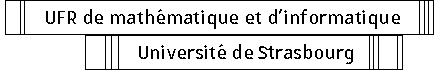
\includegraphics [width=8cm] {logo-ufr.pdf}       

    \vfill

    {
	\large
	\textsc{
	    Master d'informatique \\
	    Parcours I3D - IIRVIJ \\
		Imagerie 3D - Informatique Image Réalité Virtuelle Interaction et Jeux
	}
    }

    \bigskip\bigskip
    \bigskip\bigskip

    {\huge Travail d'Étude et de Recherche}

    \bigskip\bigskip

    % Identité de l'auteur
    {\large Pierre \textsc{EVEN}}

    % Contact mail ou téléphone   
    {\small pierre.even@etu.unistra.fr}

    \vfill

    % Titre du TER : mettez un titre utile
    {
	\huge
	\textsc{
		Segmentation d'arbre \\
	    ~ \\
	    dans un nuage de points.
	}
    }

    \vfill
    \vfill

    \today

    \vfill

    {\large TER encadré par}

    \medskip

    {
		\large Joris \textsc{Ravaglia} \small{ravaglia@unistra.fr}\\
		\large Franck \textsc{Hetroy Wheeler} \small{hetroywheeler@unistra.fr}
	}

    \bigskip

    \bigskip
\end{center}

%%%%%%%%%%%%%%%%%%%%%%%%%%%%%%%%%%%%%%%%%%%%%%%%%%%%%%%%%%%%%%%%%%%%%%%%%%%%%%
% Table des matières
%%%%%%%%%%%%%%%%%%%%%%%%%%%%%%%%%%%%%%%%%%%%%%%%%%%%%%%%%%%%%%%%%%%%%%%%%%%%%%

{
    \parskip=0pt
    \tableofcontents
}

% Page blanche entre la table des matières et le texte
\cleardoublepage

%%%%%%%%%%%%%%%%%%%%%%%%%%%%%%%%%%%%%%%%%%%%%%%%%%%%%%%%%%%%%%%%%%%%%%%%%%%%%%
% Chapitre 1
%%%%%%%%%%%%%%%%%%%%%%%%%%%%%%%%%%%%%%%%%%%%%%%%%%%%%%%%%%%%%%%%%%%%%%%%%%%%%%

%%%%%%%%%%%%%%%%%%%%%%%%%%%%%%%%%%%%%%%%%%%%%%%%%%%%%%%%%%%%%%%%%%%%%%%%%%%%%%
% Conclusion
%%%%%%%%%%%%%%%%%%%%%%%%%%%%%%%%%%%%%%%%%%%%%%%%%%%%%%%%%%%%%%%%%%%%%%%%%%%%%%

\chapter{Conclusion}
    \label{chap:conc}
